% Paquets généraux
\documentclass[a4paper,12pt,titlepage]{article}
\usepackage[T1]{fontenc}
\usepackage[utf8]{inputenc}
\usepackage[french]{babel}
\usepackage[gen]{eurosym}
%\usepackage[dvips]{graphicx}
\usepackage{fancyhdr}
\usepackage{pdfpages} 
\usepackage{multido}
\usepackage{hyperref}
%\usepackage{textcomp}
%\usepackage{aeguill}
\usepackage{schemabloc}
\usepackage[bitstream-charter]{mathdesign}
\usepackage{pstricks}
\usepackage{helvet}

\newcommand{\id}{54}
\newcommand{\nom}{Liaisons mécaniques}
\newcommand{\sequence}{04}
\newcommand{\num}{01}
\newcommand{\type}{TP}
\newcommand{\descrip}{Modélisation d'un solide. Comportement des liaisons mécaniques. Modéliser les mécanismes du laboratoire par un schéma cinématique, paramétré.}
\newcommand{\competences}{A3-C4: Analyse d'architecture et de comportement \\ &  Mod1-C1: Isolement d'un solide ou d'un système de solides \\ &  Mod2-C10-1: Modèle de solide indéformable \\ &  Mod2-C11: Modélisation géométrique et cinématique des mouvements entre solides indéformables \\ &  Mod2-C12: Modélisation cinématique des liaisons entre solides \\ &  Mod2-C15: Modélisation des actions mécaniques \\ &  Rés-C6: Utilisation d'un solveur ou d'un logiciel multi physique \\ &  Com1-C1: Différents descripteurs introduits dans le programme \\ &  Com2-C4: Outils de communication}
\newcommand{\nbcomp}{9}
\newcommand{\systemes}{Plateforme Stewart}
\newcommand{\systemessansaccent}{Plateforme Stewart}
\newcommand{\ilot}{2}
\newcommand{\ilotstr}{02}
\newcommand{\dossierilot}{\detokenize{Ilot_02 Plateforme Stewart}}
\newcommand{\imageun}{Plateforme}

\newcommand{\urlsysteme}{\href{https://www.costadoat.fr/systeme/57}{Ressources système}}
\newcommand{\matlabsimscape}{\href{https://github.com/Costadoat/Sciences-Ingenieur/raw/master/Systemes/Plateforme Stewart/Plateforme_Stewart_Simscape.zip}{Modèle Simscape}}
\newcommand{\solidworks}{\href{https://github.com/Costadoat/Sciences-Ingenieur/raw/master/Systemes/Plateforme Stewart/Plateforme_Stewart_Solidworks.zip}{Modèle Solidworks}}
\newcommand{\edrawings}{\href{https://github.com/Costadoat/Sciences-Ingenieur/raw/master/Systemes/Plateforme Stewart/Plateforme_Stewart.EASM}{Modèle eDrawings}}
\newcommand{\test}{Stewart_param1}
\newcommand{\testi}{Stewart_param2}
\newcommand{\testii}{Stewart_param3}
\newcommand{\testiii}{Stewart_param4}
\newcommand{\testiiii}{Stewart_euler}

\newcommand{\auteurun}{Renaud Costadoat}
\newcommand{\institute}{Lycée Dorian}


\usepackage{color}
\usepackage{xcolor}
\usepackage{colortbl}
\usepackage{helvet}
\renewcommand{\familydefault}{\sfdefault}
\usepackage{amsfonts}
\usepackage{amsmath}
%\usepackage{xspace}
\usepackage{varioref}
\usepackage{tabularx}
%\usepackage{floatflt}
\usepackage{graphics}
\usepackage{wrapfig}
\usepackage{textcomp}
\usepackage{tikz}
\usepackage{wrapfig}
\usepackage{gensymb}
\usepackage[european]{circuitikz}
\usetikzlibrary{babel}
\usepackage{ifthen}
\usepackage{cancel}
\usepackage{etoolbox}
\usepackage{multirow}
%\usepackage{boxedminipage}
\definecolor{gris25}{gray}{0.75}
\definecolor{bleu}{RGB}{18,33,98}
\definecolor{bleuf}{RGB}{42,94,171}
\definecolor{bleuc}{RGB}{231,239,247}
\definecolor{rougef}{RGB}{185,18,27}
\definecolor{rougec}{RGB}{255,188,204}%255,230,231
\definecolor{vertf}{RGB}{103,126,82}
\definecolor{vertc}{RGB}{220,255,191}
\definecolor{forestgreen}{rgb}{0.13,0.54,0.13}
\definecolor{blcr}{rgb}{0.59,0.69,0.84}
\definecolor{blfr}{rgb}{0.32,0.51,0.75}
\definecolor{orfr}{rgb}{0.90,0.42,0.15}
\definecolor{orcr}{rgb}{0.90,0.65,0.50}
\definecolor{orangef}{rgb}{0.659,0.269,0.072}
\definecolor{orange}{rgb}{0.58,0.35,0.063}
\definecolor{orangec}{rgb}{0.43,0.32,0.25}
\definecolor{rcorrect}{rgb}{0.6,0,0}
\definecolor{sequence}{rgb}{0.75,0.75,0.75}
\definecolor{competences}{rgb}{0.61,0.73,0.35}
\definecolor{grisf}{HTML}{222222}
\definecolor{grisc}{HTML}{636363}
\definecolor{normal}{HTML}{4087c4}
\definecolor{info}{HTML}{5bc0de}
\definecolor{success}{RGB}{92,184,92}
\definecolor{warning}{RGB}{240,173,78}
\definecolor{danger}{RGB}{217,83,79}
\hypersetup{                    % parametrage des hyperliens
    colorlinks=true,                % colorise les liens
    breaklinks=true,                % permet les retours à la ligne pour les liens trop longs
    urlcolor= blfr,                 % couleur des hyperliens
    linkcolor= orange,                % couleur des liens internes aux documents (index, figures, tableaux, equations,...)
    citecolor= forestgreen                % couleur des liens vers les references bibliographiques
    }

% Mise en page
\pagestyle{fancy}

\setlength{\hoffset}{-18pt}

\setlength{\oddsidemargin}{0pt} 	% Marge gauche sur pages impaire2s
\setlength{\evensidemargin}{0pt} 	% Marge gauche sur pages paires
\setlength{\marginparwidth}{00pt} 	% Largeur de note dans la marge
\setlength{\headwidth}{481pt} 	 	% Largeur de la zone de tête (17cm)
\setlength{\textwidth}{481pt} 	 	% Largeu\textbf{r de la zone de texte (17cm)
\setlength{\voffset}{-18pt} 		% Bon pour DOS
\setlength{\marginparsep}{7pt}	 	% Séparation de la marge
\setlength{\topmargin}{-30pt} 		% Pas de marge en haut
\setlength{\headheight}{55pt} 		% Haut de page
\setlength{\headsep}{20pt} 		% Entre le haut de page et le texte
\setlength{\footskip}{30pt} 		% Bas de\textbf{ page + séparation
\setlength{\textheight}{700pt} 		% Hauteur de l'icone zone de texte (25cm)
\setlength\fboxrule{1 pt}
\renewcommand{\baselinestretch}{1}
\setcounter{tocdepth}{1}
\newcommand{\cadre}[2]
{\fbox{
  \begin{minipage}{#1\linewidth}
   \begin{center}
    #2\\
   \end{center}
  \end{minipage}
 }
}

\newcommand{\reponse}[1][4]
{
\multido{}{#1}
{\begin{center}\makebox[0.9\linewidth]{}  \\
\begin{center}\makebox[0.9\linewidth]{\dotfill} \\ \end{center}
}}

\newcommand{\titre}[1]
{\begin{center}
\cadre{0.8}{\huge #1} 
\end{center}
}


% En tête et pied de page
\lhead{\nom}
\rhead{
\includegraphics[width=2cm]{../../img/logo}}
\lfoot{Renaud Costadoat}
\cfoot{Page \thepage}

\fancypagestyle{correction}{%
  \fancyhf{}
  \lhead{\colorbox{danger}{\begin{minipage}{0.65\paperwidth} \textcolor{white}{\textbf{Correction}} \end{minipage}} }
  \rhead{
\includegraphics[width=2cm]{../../img/logo}}
  \lfoot{Renaud Costadoat}
  \rfoot{\colorbox{danger}{\begin{minipage}{0.6\paperwidth} \begin{flushright}\textcolor{white}{\textbf{Correction}}\end{flushright} \end{minipage}} }}

\renewcommand{\footrulewidth}{0.4pt}

\usepackage{eso-pic}
\newcommand{\BackgroundPic}{%
\put(0,0){%
\parbox[b][\paperheight]{\paperwidth}{%
\vfill
\begin{center}
\hspace{0.5cm}\vspace{0.5cm}

\includegraphics[width=\paperwidth,height=\paperheight,%
keepaspectratio]{../../img/fond3}%
\end{center}
\vfill
}}}

\newcommand{\BackgroundPicdeux}{%
\put(25,-30){%
\parbox[b][\paperheight]{\paperwidth}{%
\vfill
\begin{center}
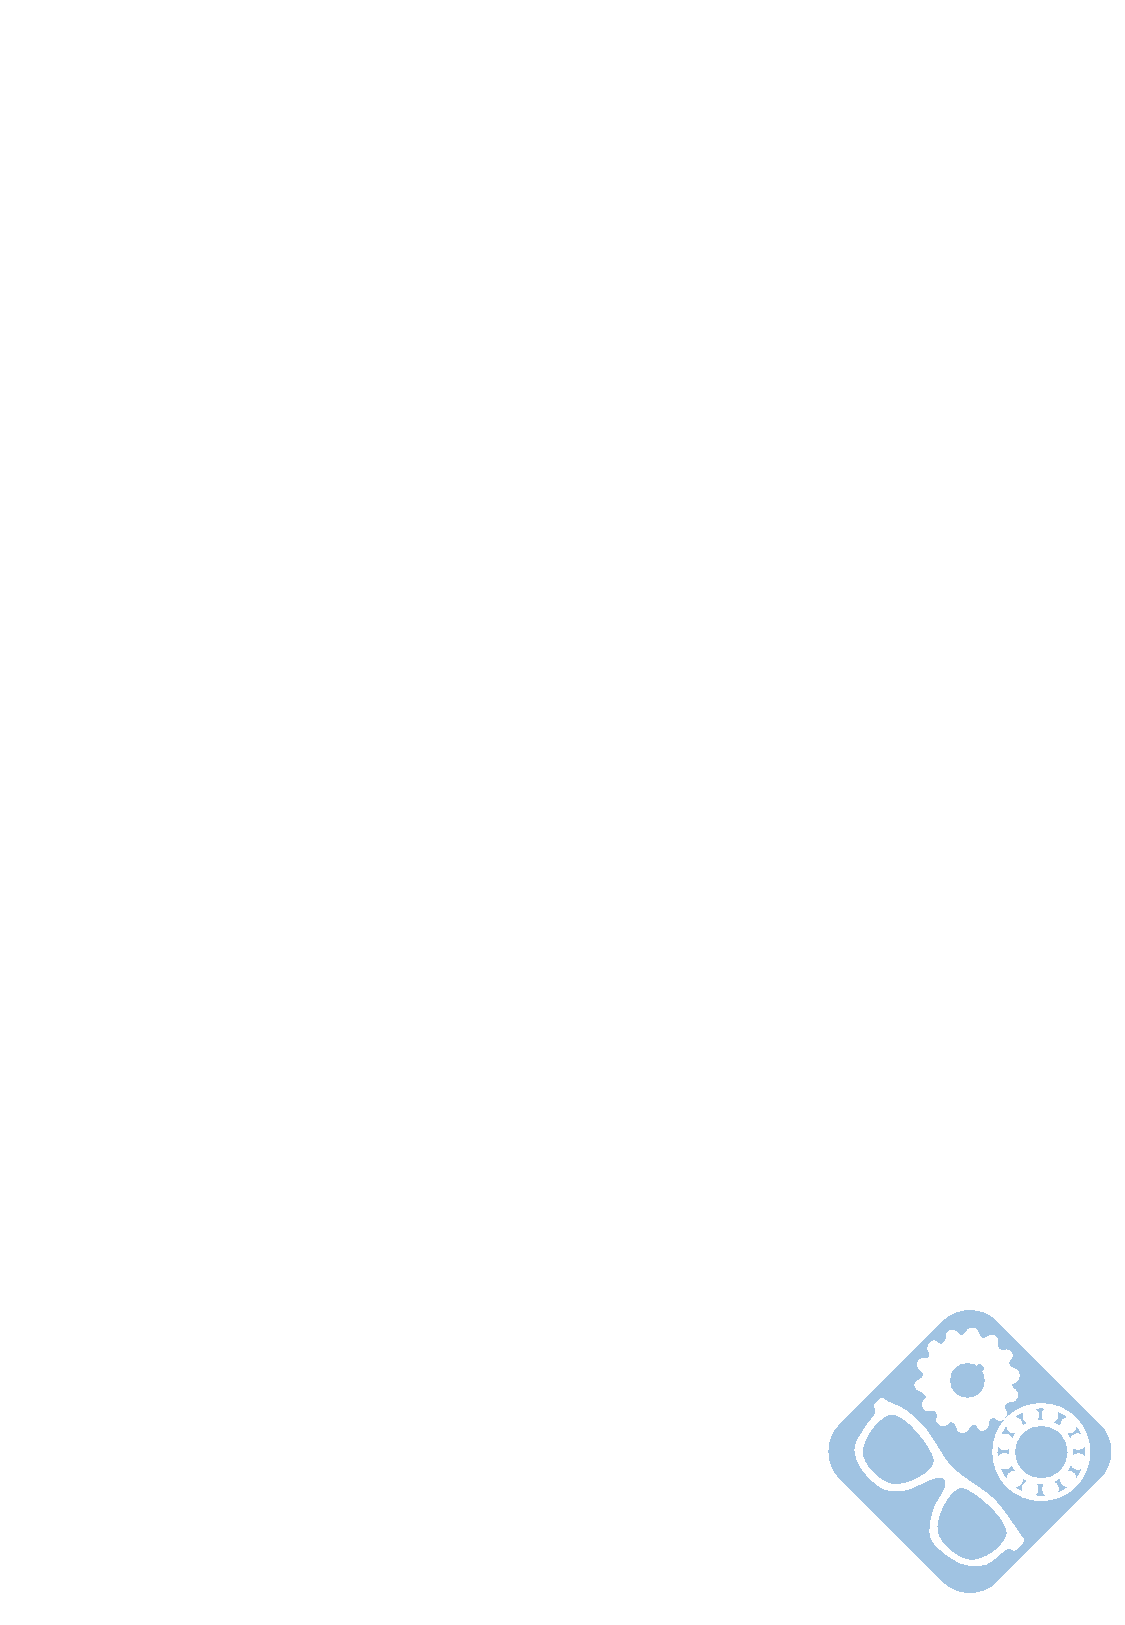
\includegraphics[width=\paperwidth,height=\paperheight,%
keepaspectratio]{../../img/fond4}%
\end{center}
\vfill
}}}

\begin{document}

\AddToShipoutPicture{\BackgroundPicdeux}

\pagestyle{fancy}

\section{Le manège à sensations XXL}

Le système étudié ici est un manège appelé \og Manège à sensations XXL \fg. L'étude consiste à déterminer l'accélération subite par une personne, et de vérifier que la limite supportable (sans déconfort) par l'homme d'une valeur de 2g n'est pas dépassée...

\begin{figure}[htbp]
\begin{minipage}[c]{.48\linewidth}
\begin{center}
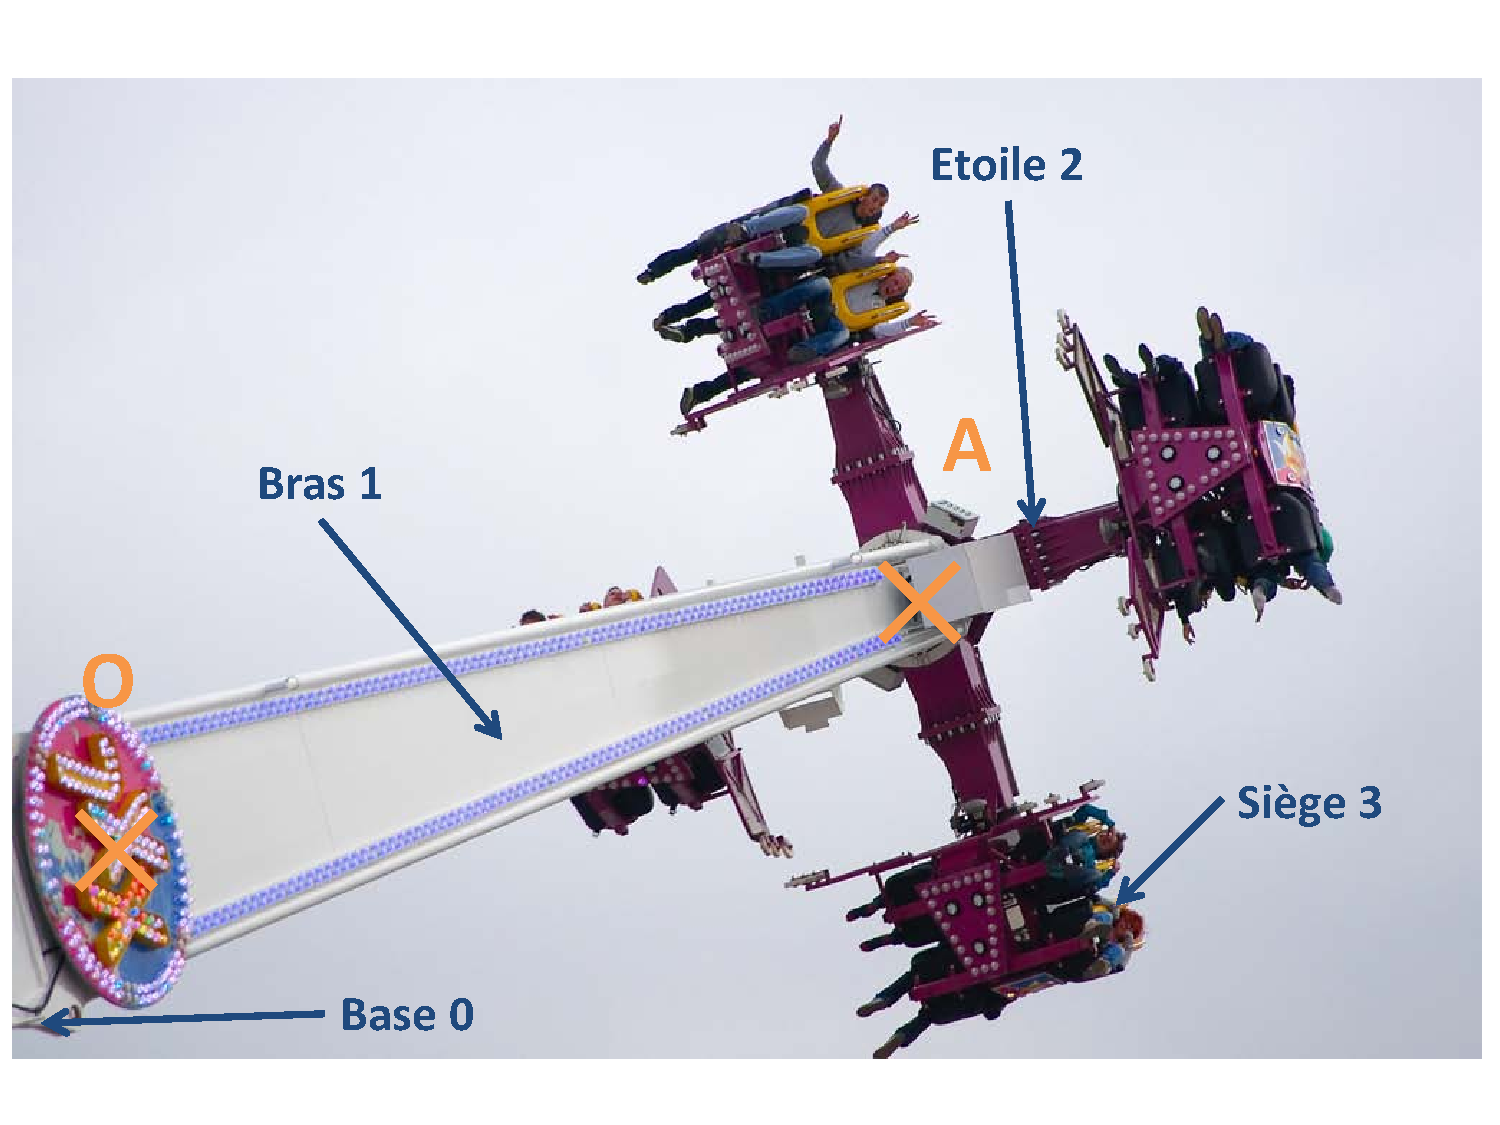
\includegraphics[width=\linewidth]{img/Manege1.pdf}
\caption{Vue du bras du ménège}
\label{fig:image1}
\end{center}
\end{minipage}
\hfill
\begin{minipage}[c]{.48\linewidth}
\begin{center}
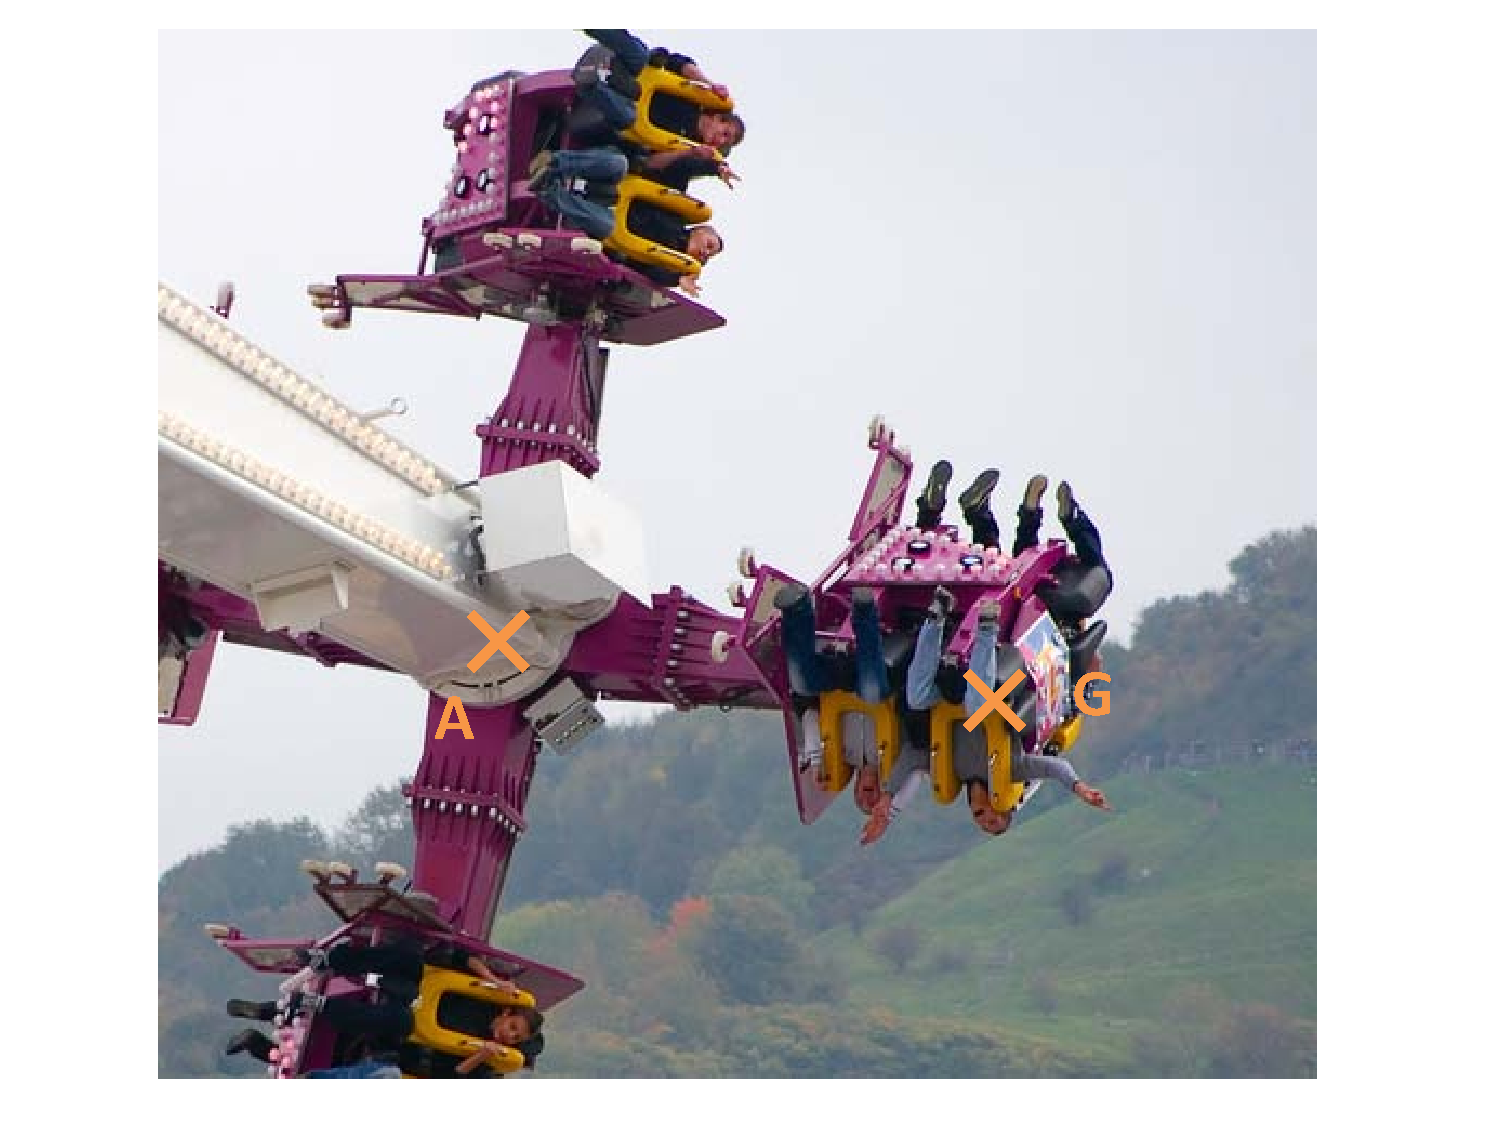
\includegraphics[width=\linewidth]{img/Manege2.pdf}
\caption{Vue de l'étoile}
\label{fig:image2}
\end{center}
\end{minipage}
\end{figure}

Ce système est constitué de quatre solides :
\begin{itemize}
 \item  La Base 0, de repère associé $R_O(\overrightarrow{x_0},\overrightarrow{y_0},\overrightarrow{z_0})$, fixe par rapport à la terre telle que l'axe $(O, \overrightarrow{z_0})$, soit dirigé suivant la verticale ascendante,
 \item Le Bras 1, de repère associé $R_1(\overrightarrow{x_1},\overrightarrow{y_1},\overrightarrow{z_1})$, en mouvement de rotation, d'axe $(O, \overrightarrow{x_0})$ par rapport à l base et tel que $\alpha=(\overrightarrow{y_0},\overrightarrow{y_1})=(\overrightarrow{z_0},\overrightarrow{z_1})$,
 \item L'étoile 2, de repère associé $R_2(\overrightarrow{x_2},\overrightarrow{y_2},\overrightarrow{z_2})$, en mouvement de rotation d'axe $(A, \overrightarrow{z_1})$ par rapport au plateau 1 tel que $\overrightarrow{OA}=a.\overrightarrow{z_1}$ (avec a constant), et $\beta=(\overrightarrow{x_1},\overrightarrow{x_2})=(\overrightarrow{y_1},\overrightarrow{y_2})$,
 \item Le siège 3 (lié à la personne, de repère associé $R_3(\overrightarrow{x_3},\overrightarrow{y_3},\overrightarrow{z_3})$, en mouvement de rotation d'axe $(A, \overrightarrow{x_2})$, avec $\gamma=(\overrightarrow{y_2},\overrightarrow{y_3})=(\overrightarrow{z_2},\overrightarrow{z_3})$
 \item La position de la personne est définie par son centre de gravité G, qui appartient au siège 3 et avec $\overrightarrow{AG}=b.\overrightarrow{x_2}+c.\overrightarrow{z_3}$ (avec b et c constants).
\end{itemize}

\paragraph{Question 1:} Déterminer les trajectoires $T_{G \in 3/2}$, $T_{G \in 2/1}$, $T_{G \in 1/0}$ et $T_{G \in 3/0}$.

\paragraph{Question 2:} Réaliser un schéma cinématique de l'ensemble.

\paragraph{Question 3:} Réaliser des figures planes illustrant les 3 paramètres d'orientation.

\paragraph{Question 4:} En déduire sous chaque figure, le vecteur rotation traduisant la figure.

\paragraph{Question 5:} En déduire, $\overrightarrow{\Omega_{3/0}}$.

\paragraph{Question 6:} Les 3 angles $\alpha$, $\beta$ et $\gamma$ sont-ils les angles d'Euler ?

\textit{Remarque : Le mouvement d'un solide par rapport à un référentiel fait intervenir 6 paramètres, qui sont, par exemple, les trois coordonnées décrivant la position de son centre de masse (ou d'un point quelconque du solide) et trois angles, nommés les angles d'Euler. Ces paramètres doivent permettre de décrire la position d'un point et être indépendants.}


\paragraph{Question 7:} Déterminer les vecteurs vitesses $\overrightarrow{V_{G \in 3/2}}$, $\overrightarrow{V_{G \in 2/1}}$, $\overrightarrow{V_{G \in 1/0}}$ et $\overrightarrow{V_{G \in 3/0}}$ (Vérifier l'homogénéité des résultats).

\paragraph{Question 8:} Déterminer le vecteur accélération $\overrightarrow{\Gamma_{G \in 3/0}}$ (Vérifier l'homogénéité du résultat).

\newpage

\section{Camion benne}

Un camion à benne basculante ou camion benne est un type de camion utilisé généralement pour le transport de matériaux en vrac tel que du sable, du gravier, de terre ou de gravats.

Un camion à benne basculante est ordinairement équipé d'un vérin hydraulique qui soulève l'avant de la benne à la demande, permettant ainsi de la vider par gravité, en partie ou totalité, que le camion soit immobile ou en déplacement.

\begin{figure}[htbp]
\begin{minipage}[c]{.48\linewidth}
\begin{center}
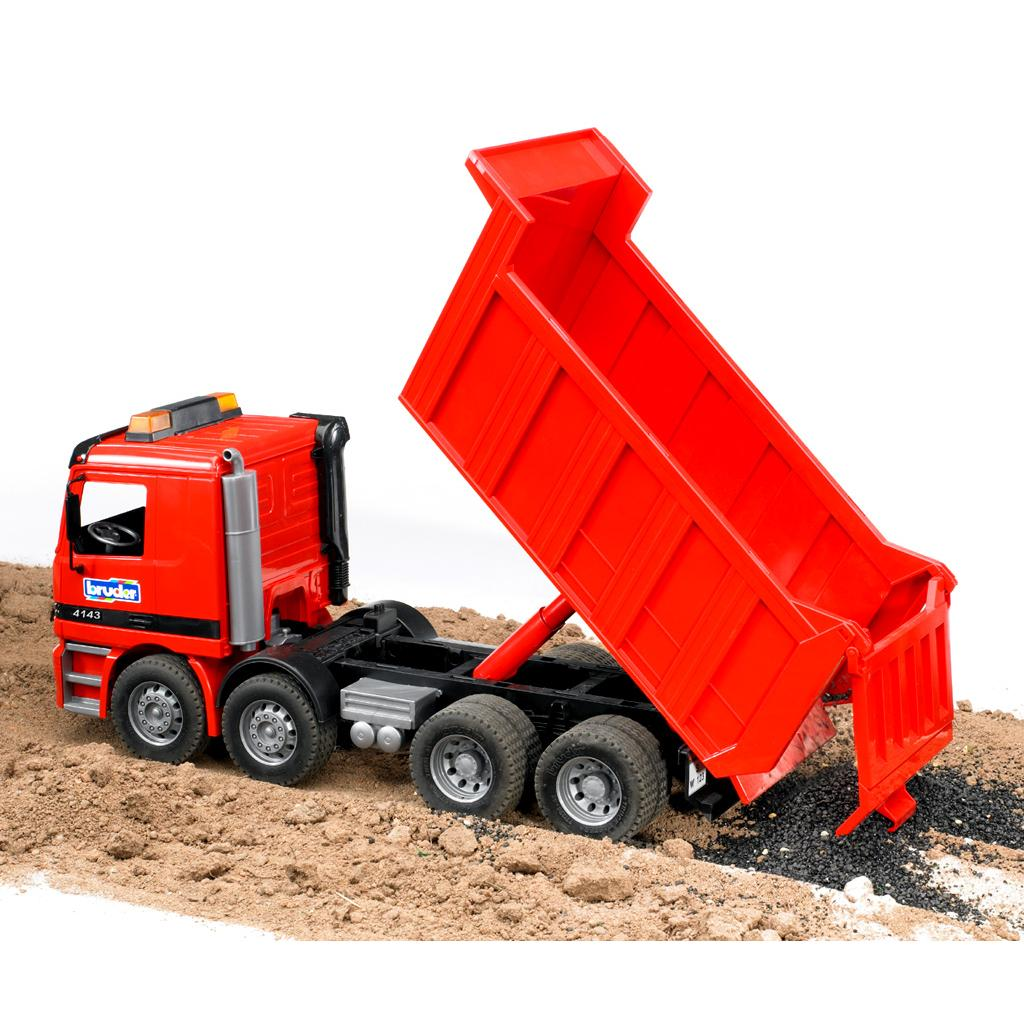
\includegraphics[width=\linewidth]{img/camion-benne.jpg}
\caption{Camion benne en extension}
\label{fig:image3}
\end{center}
\end{minipage}
\hfill
\begin{minipage}[c]{.48\linewidth}
Soit $R_O(\overrightarrow{x_0},\overrightarrow{y_0},\overrightarrow{z_0})$ un repère lié au châssis 0 d'un camion benne.
Soient $R_1(\overrightarrow{x_1},\overrightarrow{y_1},\overrightarrow{z_1})$ un repère lié à la benne 1 et $R_2(\overrightarrow{x_2},\overrightarrow{y_2},\overrightarrow{z_2})$ un repère lié à la tige 2
et au corp 3 du vérin hydraulique.

Le mécanisme étudié est considéré dans le plan $(\overrightarrow{x_0},\overrightarrow{y_0})$. Le corps 1 a un mouvement de rotation d'axe $(O, \overrightarrow{z_0})$ par rapport au châssis 0 avec $\alpha=(\overrightarrow{x_0},\overrightarrow{x_1})=(\overrightarrow{y_0},\overrightarrow{y_1})$. La tige 2 à un mouvement de rotation d'axe $(B, \overrightarrow{z_0})$ par rapport à la benne 1 et le corp 3 du vérin un mouvement de rotation d'axe $(A, \overrightarrow{z_0})$ par rapport au châssis 0 du camion benne.

La tige 2 a un mouvement de translation rectiligne de direction $\overrightarrow{y_2}$ par rapport au corps 3 du vérin. On pose $\overrightarrow{AB}=\lambda.\overrightarrow{y_2}$ ($\lambda$ varie).
\end{minipage}
\end{figure}

\paragraph{Question 1:} Déterminer les trajectoires $T_{B \in 3/2}$, $T_{B \in 1/0}$.

\paragraph{Question 2:} Réaliser un schéma cinématique de l'ensemble.

\paragraph{Question 3:} Réaliser des figures planes illustrant le paramètre d'orientation.

\paragraph{Question 4:} Déterminer, $\overrightarrow{\Omega_{1/0}}$.

\paragraph{Question 5:} Déterminer les vecteurs vitesses $\overrightarrow{V_{B \in 3/2}}$, $\overrightarrow{V_{B \in 1/0}}$. (Vérifier l'homogénéité des résultats).

\paragraph{Question 6:} Déterminer le vecteur accélération $\overrightarrow{\Gamma_{B \in 1/0}}$ (Vérifier l'homogénéité du résultat).

\newpage

~\

\newpage

\section{Bras manipulateur}

Un bras manipulateur est le bras d'un robot généralement programmable, avec des fonctions similaires à un bras humain. Les liens de ce manipulateur sont reliés par des axes permettant, soit du mouvement de rotation (comme dans un robot articulé) ou de translation (linéaire) de déplacement.

\begin{figure}[htbp]
\begin{minipage}[c]{.48\linewidth}
\begin{center}
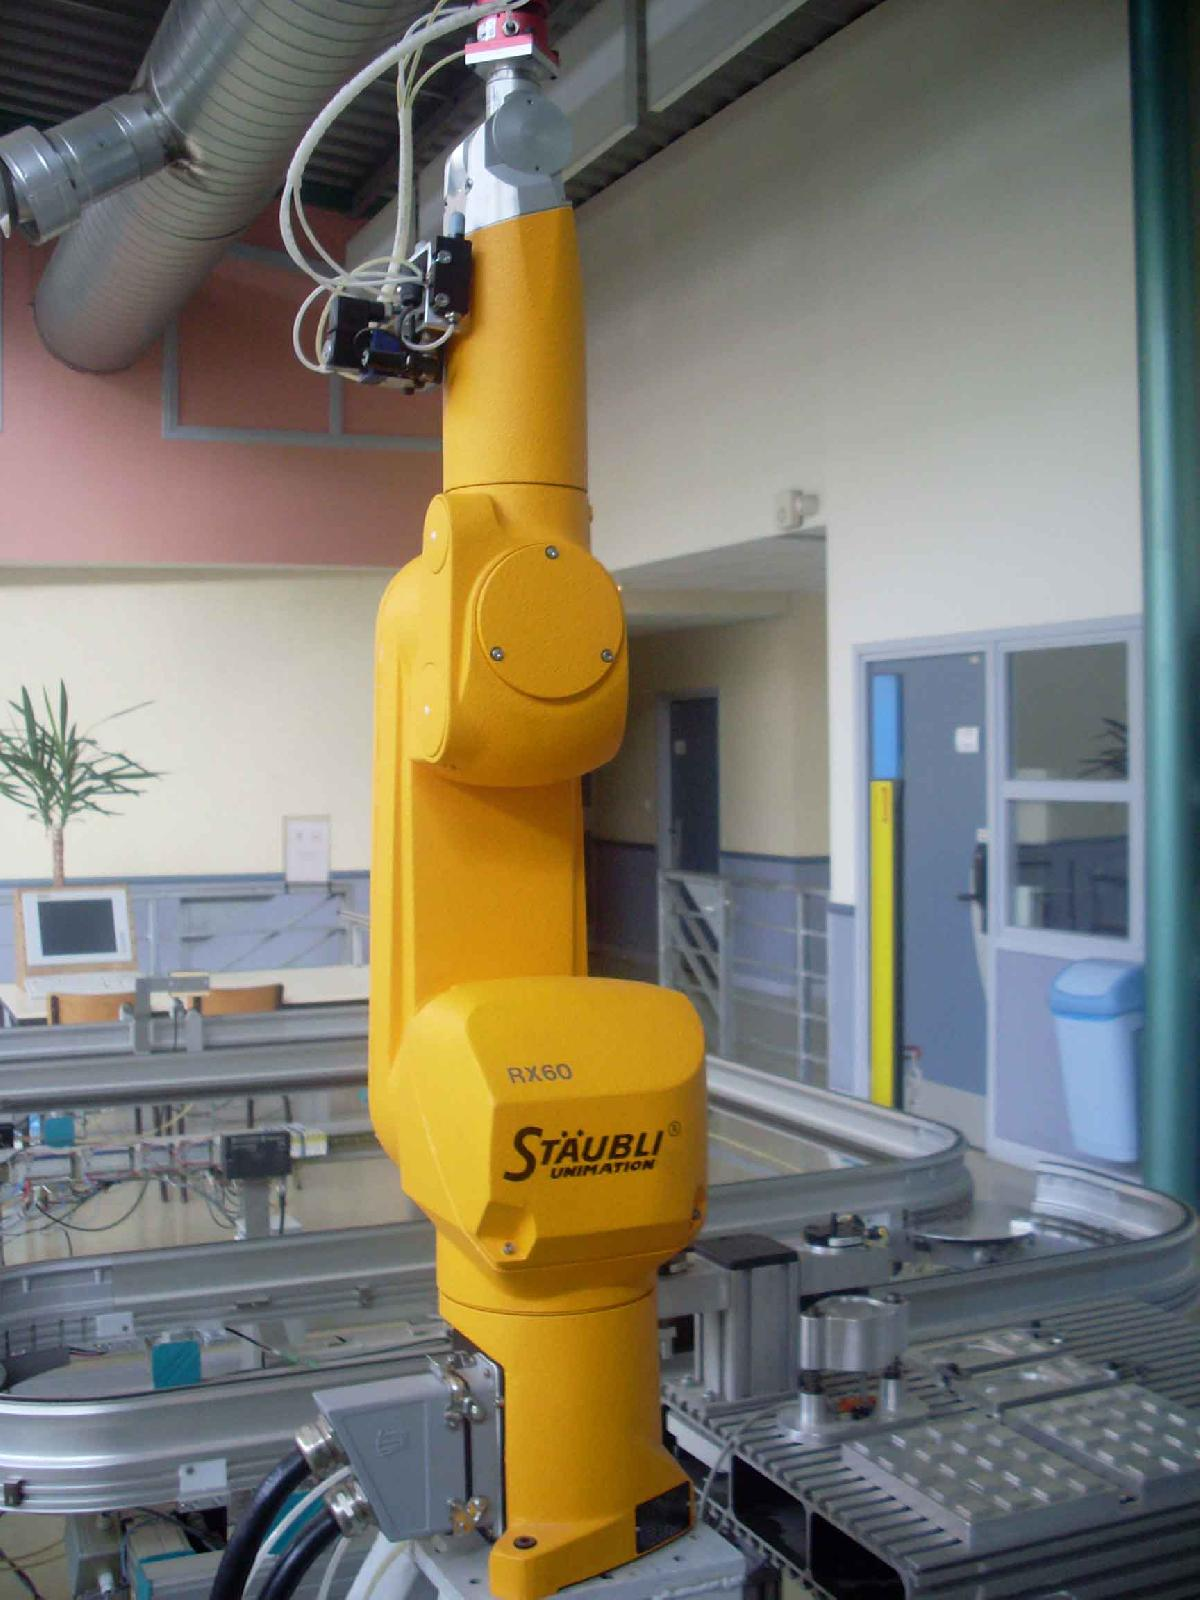
\includegraphics[width=\linewidth]{img/robot.jpg}
\caption{Exemple de bras manipulateur}
\label{fig:image4}
\end{center}
\end{minipage}
\hfill
\begin{minipage}[c]{.48\linewidth}
\begin{center}
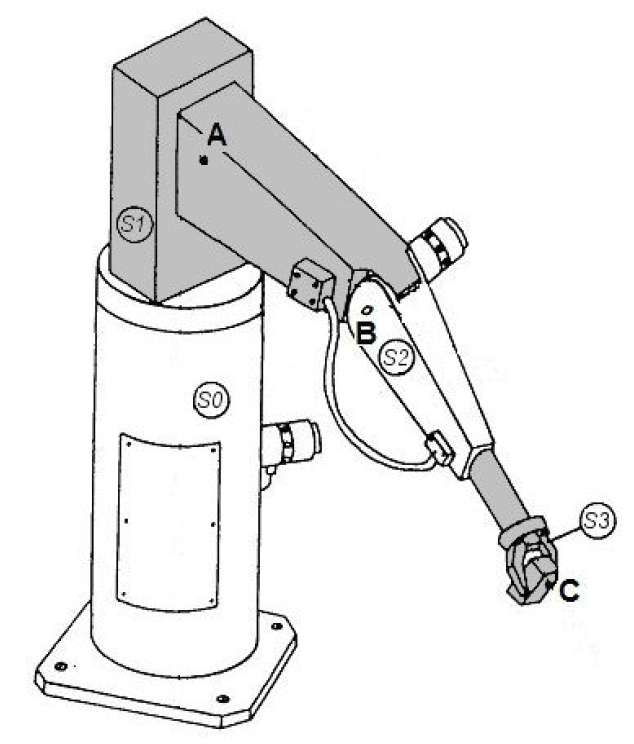
\includegraphics[width=\linewidth]{img/bras.png}
\caption{Bras étudié}
\label{fig:image5}
\end{center}
\end{minipage}
\end{figure}

Le schéma de droite ci-dessus représente un bras manipulateur permettant de déplacer des objets.
Ce mécanisme est constitué de :
\begin{itemize}
 \item Un bâti S0,
 \item Un solide S1 entraîné en rotation par un moteur M1,
 \item Un solide S2 entraîné en rotation par un moteur M2,
 \item Un solide S3 entraîné en translation par un vérin V1,
 \item Une pince située à l'extrémité du vérin permettant de saisir l'objet.
\end{itemize}

\begin{itemize}
 \item Le mouvement de S1 par rapport à S0 est une rotation d'axe $(A, \overrightarrow{z_0})$, 
 \item Le mouvement de S2 par rapport à S1 est une rotation d'axe $(B, \overrightarrow{x_1})$,
 \item Le mouvement de S3 par rapport à S2 est une translation rectiligne de direction $\overrightarrow{z_2}$.
\end{itemize}

On pose $\overrightarrow{AB}=a.\overrightarrow{y_1}$ (a étant une constante).

\paragraph{Question 1:} Déterminer les trajectoires $T_{C \in 3/2}$, $T_{C \in 2/1}$ et $T_{C \in 1/0}$,
\paragraph{Question 2:} Proposer un paramétrage intelligent du système,
\paragraph{Question 3:} Réaliser des figures planes illustrant les paramètres d'orientation,
\paragraph{Question 4:} Déterminer les vecteurs vitesses $\overrightarrow{V_{C \in 3/2}}$, $\overrightarrow{V_{C \in 2/1}}$, $\overrightarrow{V_{C \in 1/0}}$ et $\overrightarrow{V_{C \in 3/0}}$,
\paragraph{Question 5:} Déterminer le vecteur accélération $\overrightarrow{\Gamma_{C \in 3/0}}$.

\newpage

\section{Basculeur de bobines}

\subsection{Présentation}

\begin{figure}[!h]
 \begin{minipage}{0.5\linewidth}
 Pour les machines consommant des films (étiquettes, plastique pour regrouper des produits, cellophanage de produit unitaire (exemple parfumerie)), les bobines doivent être posées souvent en hauteur ou au ras du sol.
 
 L'objectif de cette étude est de déterminer la vitesse de déplacement de la bobine en fonction de la vitesse d'entrée/sortie du vérin de pilotage.
 \end{minipage}
 \hfill
 \begin{minipage}{0.4\linewidth}
  \centering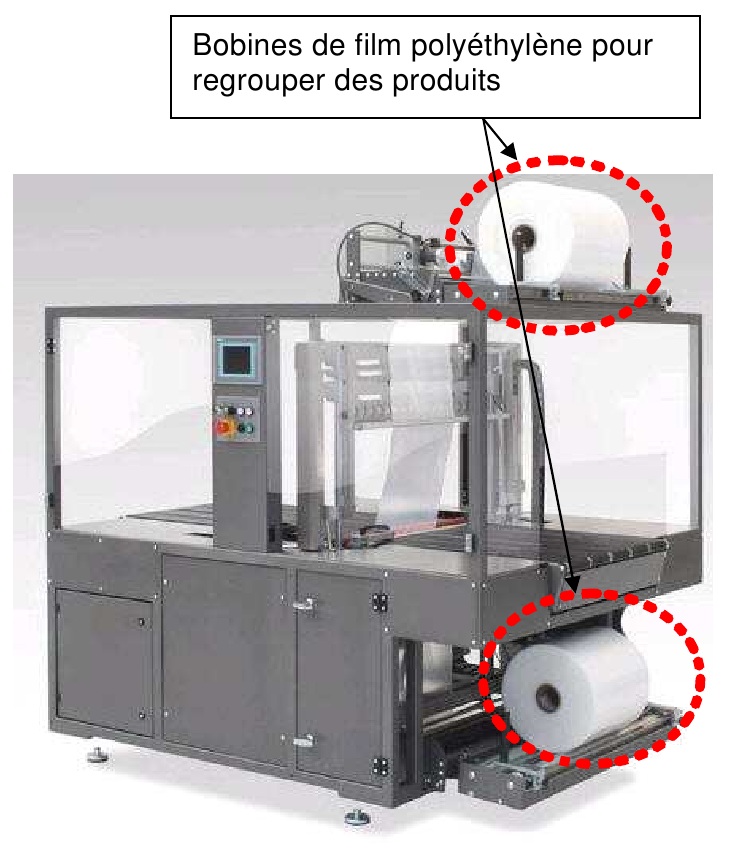
\includegraphics[width=0.9\linewidth]{img/bobine.png}
 \end{minipage}
\end{figure}

\subsection{Calcul cinématique}

Données:
\begin{figure}[!h]
 \begin{minipage}{0.45\linewidth}
\begin{itemize}
 \item $\overrightarrow{AG_2}=\overrightarrow{CG}=(l+l_0).\overrightarrow{x_2}$,
 \item $l_0$ : longueur minimale du vérin,
 \item $l$ : allongement du vérin,
 \item $\overrightarrow{DG_2}=a.\overrightarrow{x_4}$,
 \item $\overrightarrow{AD}=d.\overrightarrow{y_0}$,
\end{itemize}
 \end{minipage}
\hfill
 \begin{minipage}{0.45\linewidth}
\begin{itemize}
 \item $\overrightarrow{DJ_2}=b.\overrightarrow{x_4}-c.\overrightarrow{y_4}$,
 \item $\overrightarrow{J_2N}=e.\overrightarrow{x_2}-f.\overrightarrow{y_2}$,
 \item $\theta_{21}=(\overrightarrow{x_0},\overrightarrow{x_2})=(\overrightarrow{y_0},\overrightarrow{y_2})$,
 \item $\theta_{41}=(\overrightarrow{x_0},\overrightarrow{x_4})=(\overrightarrow{y_0},\overrightarrow{y_4})$,
 \item $\theta_{61}=(\overrightarrow{x_0},\overrightarrow{x_6})=(\overrightarrow{y_0},\overrightarrow{y_6})$.
\end{itemize}
 \end{minipage}
\end{figure}

\paragraph{Question 1:} Fermeture géométrique

Déterminer:
\begin{itemize}
 \item $\overrightarrow{AG_2}$ dans le repère $(\overrightarrow{x_0},\overrightarrow{y_0},\overrightarrow{z_0})$,
 \item $\overrightarrow{DG_2}$ dans le repère $(\overrightarrow{x_0},\overrightarrow{y_0},\overrightarrow{z_0})$,
 \item $\overrightarrow{AD}$ dans le repère $(\overrightarrow{x_0},\overrightarrow{y_0},\overrightarrow{z_0})$.
\end{itemize}

Ecrire l'équation de fermeture géométrique, la projeter sur $\overrightarrow{x_0}$ et $\overrightarrow{y_0}$, montrer que l'on obtient les équations suivantes:
\begin{itemize}
 \item $cos\theta_{21}.(l+l_0)=a.cos\theta_{41}$,
 \item $sin\theta_{21}.(l+l_0)=d+a.sin\theta_{41}$.
\end{itemize}

\paragraph{Question 2:} Mouvement de 3

Déterminer $\overrightarrow{V_{A \in S2/S1}}$, puis $\overrightarrow{V_{G_2 \in S2/S1}}$ en fonction de $l$, $l_0$ et $\dot{\theta_{21}}$ sur $\overrightarrow{y_2}$.

Déterminer $\overrightarrow{V_{G_2 \in S3/S2}}$ en fonction de $\dot{l}$ sur $\overrightarrow{x_2}$.

En déduire $\overrightarrow{V_{G_2 \in S3/S1}}$ en fonction de $l$, $l_0$, $\dot{l}$ et $\dot{\theta_{21}}$ sur $\overrightarrow{x_2}$ et $\overrightarrow{y_2}$.

\paragraph{Question 3:} Mouvement de 4

Déterminer $\overrightarrow{V_{D \in S4/S1}}$, puis $\overrightarrow{V_{G_2 \in S4/S1}}$ en fonction de $a$ et $\dot{\theta_{41}}$ sur $\overrightarrow{y_4}$.

Montrer que $\dot{l}.\overrightarrow{x_2}+(l_0+l).\dot{\theta_{21}}.\overrightarrow{y_2}=a.\dot{\theta_{41}}.\overrightarrow{y_4}$.

~\

Projeter cette équation sur $\overrightarrow{x_0}$ et $\overrightarrow{y_0}$.

On donne les relations trigonométriques suivantes:
\begin{itemize}
 \item $a.cos\theta_{41}=(l+l_0).cos\theta_{21}$,
 \item $d+a.sin\theta_{41}=(l+l_0).sin\theta_{21}$.
\end{itemize}

A partir des projections suivantes et des relations trigonométriques, montrer que:
\begin{itemize}
 \item $\dot{l}.\frac{a}{l+l_0}.cos\theta_{41}-(d+a.sin\theta_{41}).\dot{\theta_{21}}+a.sin\theta_{41}.\dot{\theta_{41}}=0$,
 \item $\dot{l}.\frac{d+a.sin\theta_{41}}{l+l_0}+a.cos\theta_{41}.\dot{\theta_{21}}-a.cos\theta_{41}.\dot{\theta_{41}}=0$.
\end{itemize}

En déduire $\dot{\theta_{21}}$ en fonction de $a$, $d$, $l$, $l_0$, $\theta_{41}$, $\dot{l}$ et $\dot{\theta_{41}}$.

Puis, $\dot{\theta_{41}}$ en fonction de $a$, $d$, $l$, $l_0$, $\theta_{41}$ et $\dot{l}$.

~\

Cela nous permet de calculer $\overrightarrow{\Omega_{S4/S1}}$ en fonction de la position du mécanisme et de la vitesse de sortie du vérin. Pour la suite, on prendra : $\overrightarrow{\Omega_{S4/S1}}=\dot{\theta_{41}}.\overrightarrow{z_0}$

\paragraph{Question 4:} Mouvement de 6

A partir de $\overrightarrow{\Omega_{S4/S1}}$ et de la valeur de $\overrightarrow{V_{D \in S4/S1}}$ calculée précédemment, déterminer $\overrightarrow{V_{J_2 \in S4/S1}}$, puis $\overrightarrow{V_{J_2 \in S6/S1}}$.

Un capteur permet de déterminer la vitesse de rotation $\dot{\theta_{61}}$.

Donner alors la vitesse $\overrightarrow{V_{N \in S6/S1}}$, en fonction de $b$, $c$, $e$, $f$, $\dot{\theta_{41}}$ et $\dot{\theta_{61}}$ projetée sur $\overrightarrow{x_2}$, $\overrightarrow{y_2}$, $\overrightarrow{x_4}$ et $\overrightarrow{y_4}$.

Afin de garantir la sécurité des employés, on souhaite connaître, afin de la limiter la norme de la composante horizontale de la vitesse du point N de S6 par rapport à S1. Quels calculs nécessaires faut-il faire? (Ne pas effectuer les calculs écrire simplement la méthode).

\begin{figure}[!h]
 \begin{minipage}{0.4\linewidth}
  \centering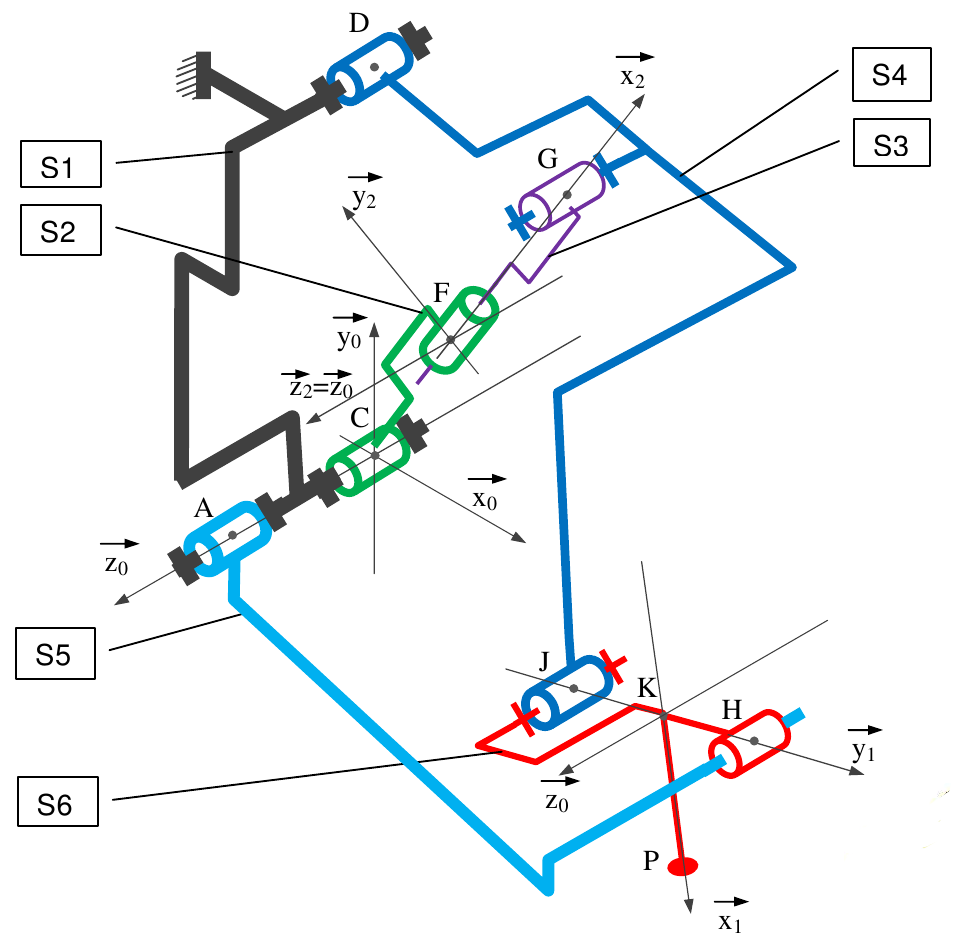
\includegraphics[width=0.9\linewidth]{img/basculeur_cin.png}
 \end{minipage}
 \hfill
 \begin{minipage}{0.58\linewidth}
  \centering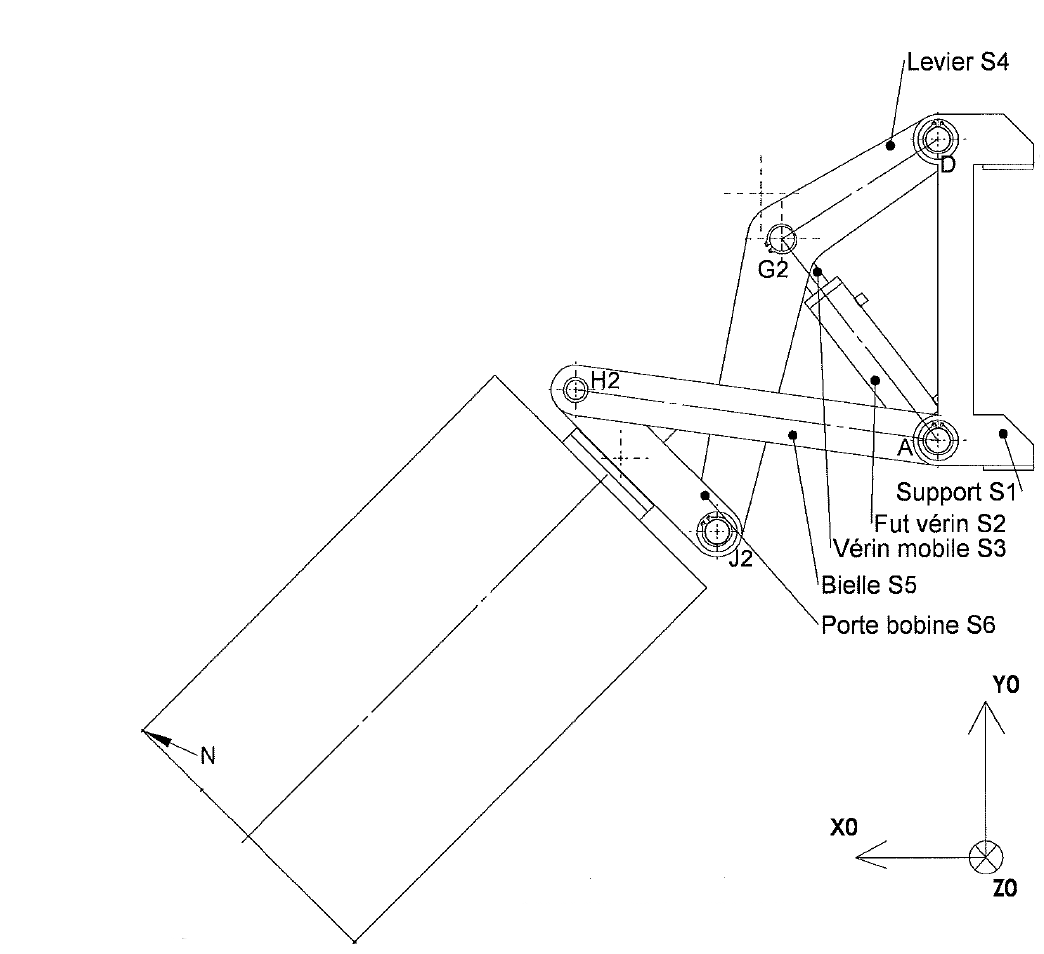
\includegraphics[width=0.9\linewidth]{img/basculeur_reduc.png}
 \end{minipage}
\end{figure}

\section{Pompe à pétrole}

\begin{figure}[!h]
\begin{minipage}[c]{.6\linewidth}
Ce type de pompe à pétrole est utilisé partout dans le monde lorsque la pression de la nappe est insuffisante pour l'extraction et qu'une action de pompage est indispensable.
\end{minipage}
\hfill
\begin{minipage}[c]{.35\linewidth}
\begin{center}
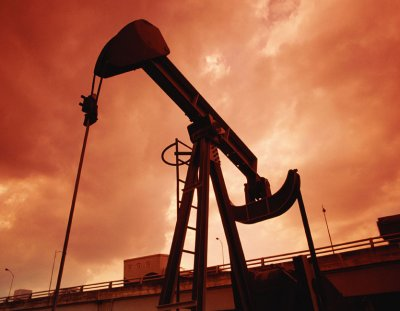
\includegraphics[width=\linewidth]{img/pompe-petrole.jpg}
\caption{Pompe à pétrole}
\label{fig:image1}
\end{center}
\end{minipage}
\end{figure}

Un moteur est installé génère le mouvement de rotation de la manivelle. Il tourne à une vitesse $\|\overrightarrow{\Omega_{1/0}}\|=15 tr.min^{-1}$.

Les dimensions suivantes sont nécessaires à la résolution:

$AB = 570mm$, $BC = 2640mm$, $CD = 2310mm$, $DE = 3400mm$.

\paragraph{Question 1:} Déterminer $\overrightarrow{V_{B \in 1/0}}$. En déduire $\overrightarrow{V_{B \in 2/0}}$.

\paragraph{Question 2:} Déterminer la direction de $\overrightarrow{V_{C \in 3/0}}$. En déduire celle de $\overrightarrow{V_{C \in 2/0}}$.

\paragraph{Question 3:} Déterminer la norme de $\overrightarrow{V_{C \in 2/0}}$. En déduire celle de $\overrightarrow{V_{C \in 3/0}}$.

\paragraph{Question 4:} En déduire $\overrightarrow{V_{N \in 3/0}}$. Puis la vitesse de déplacement du piston $\overrightarrow{V_{E \in 5/0}}$

\newpage

\begin{figure}[!h]
\begin{center}
\vspace{5cm}
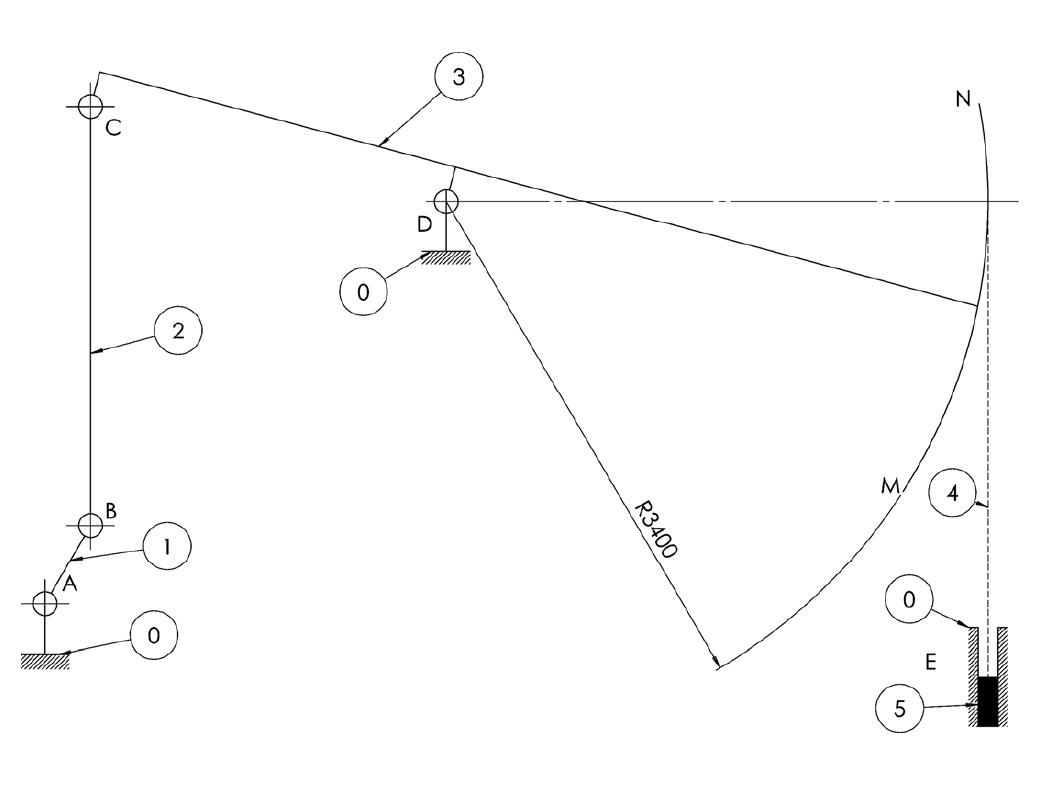
\includegraphics[width=0.8\linewidth]{img/pompe2.png}
\vspace{5cm}
\caption{Document réponse}
\label{fig:image2}
\end{center}
\end{figure}

\newpage

\section{Presse courte excentrique}

\begin{figure}[!h]
\begin{minipage}[c]{.6\linewidth}
Une presse, figure \ref{fig:image3}, permet d'appliquer de très gros efforts sur une pièce afin de la mettre en forme grâce à des déformations plastiques.

La figure \ref{fig:image4} représente une presse courte à excentrique de 2 500 tonnes dont la cadence est de 3 000 pièces à l'heure (50 coups par minute).

La presse se compose d'un moteur qui entraîne un volant d'inertie, le volant entraînant l'arbre à excentrique 1 (excentricité e = OA = 200mm, O = axe de l'arbre, A = axe de l'excentrique).
Le coulisseau porte-matrice 3 est ensuite mis en mouvement par l'intermédiaire de la coulisse 2 articulée en A sur l'excentrique 1. La liaison entre le bâti de la presse 0 et l'excentrique est une liaison pivot.
\end{minipage}
\hfill
\begin{minipage}[c]{.35\linewidth}
\begin{center}
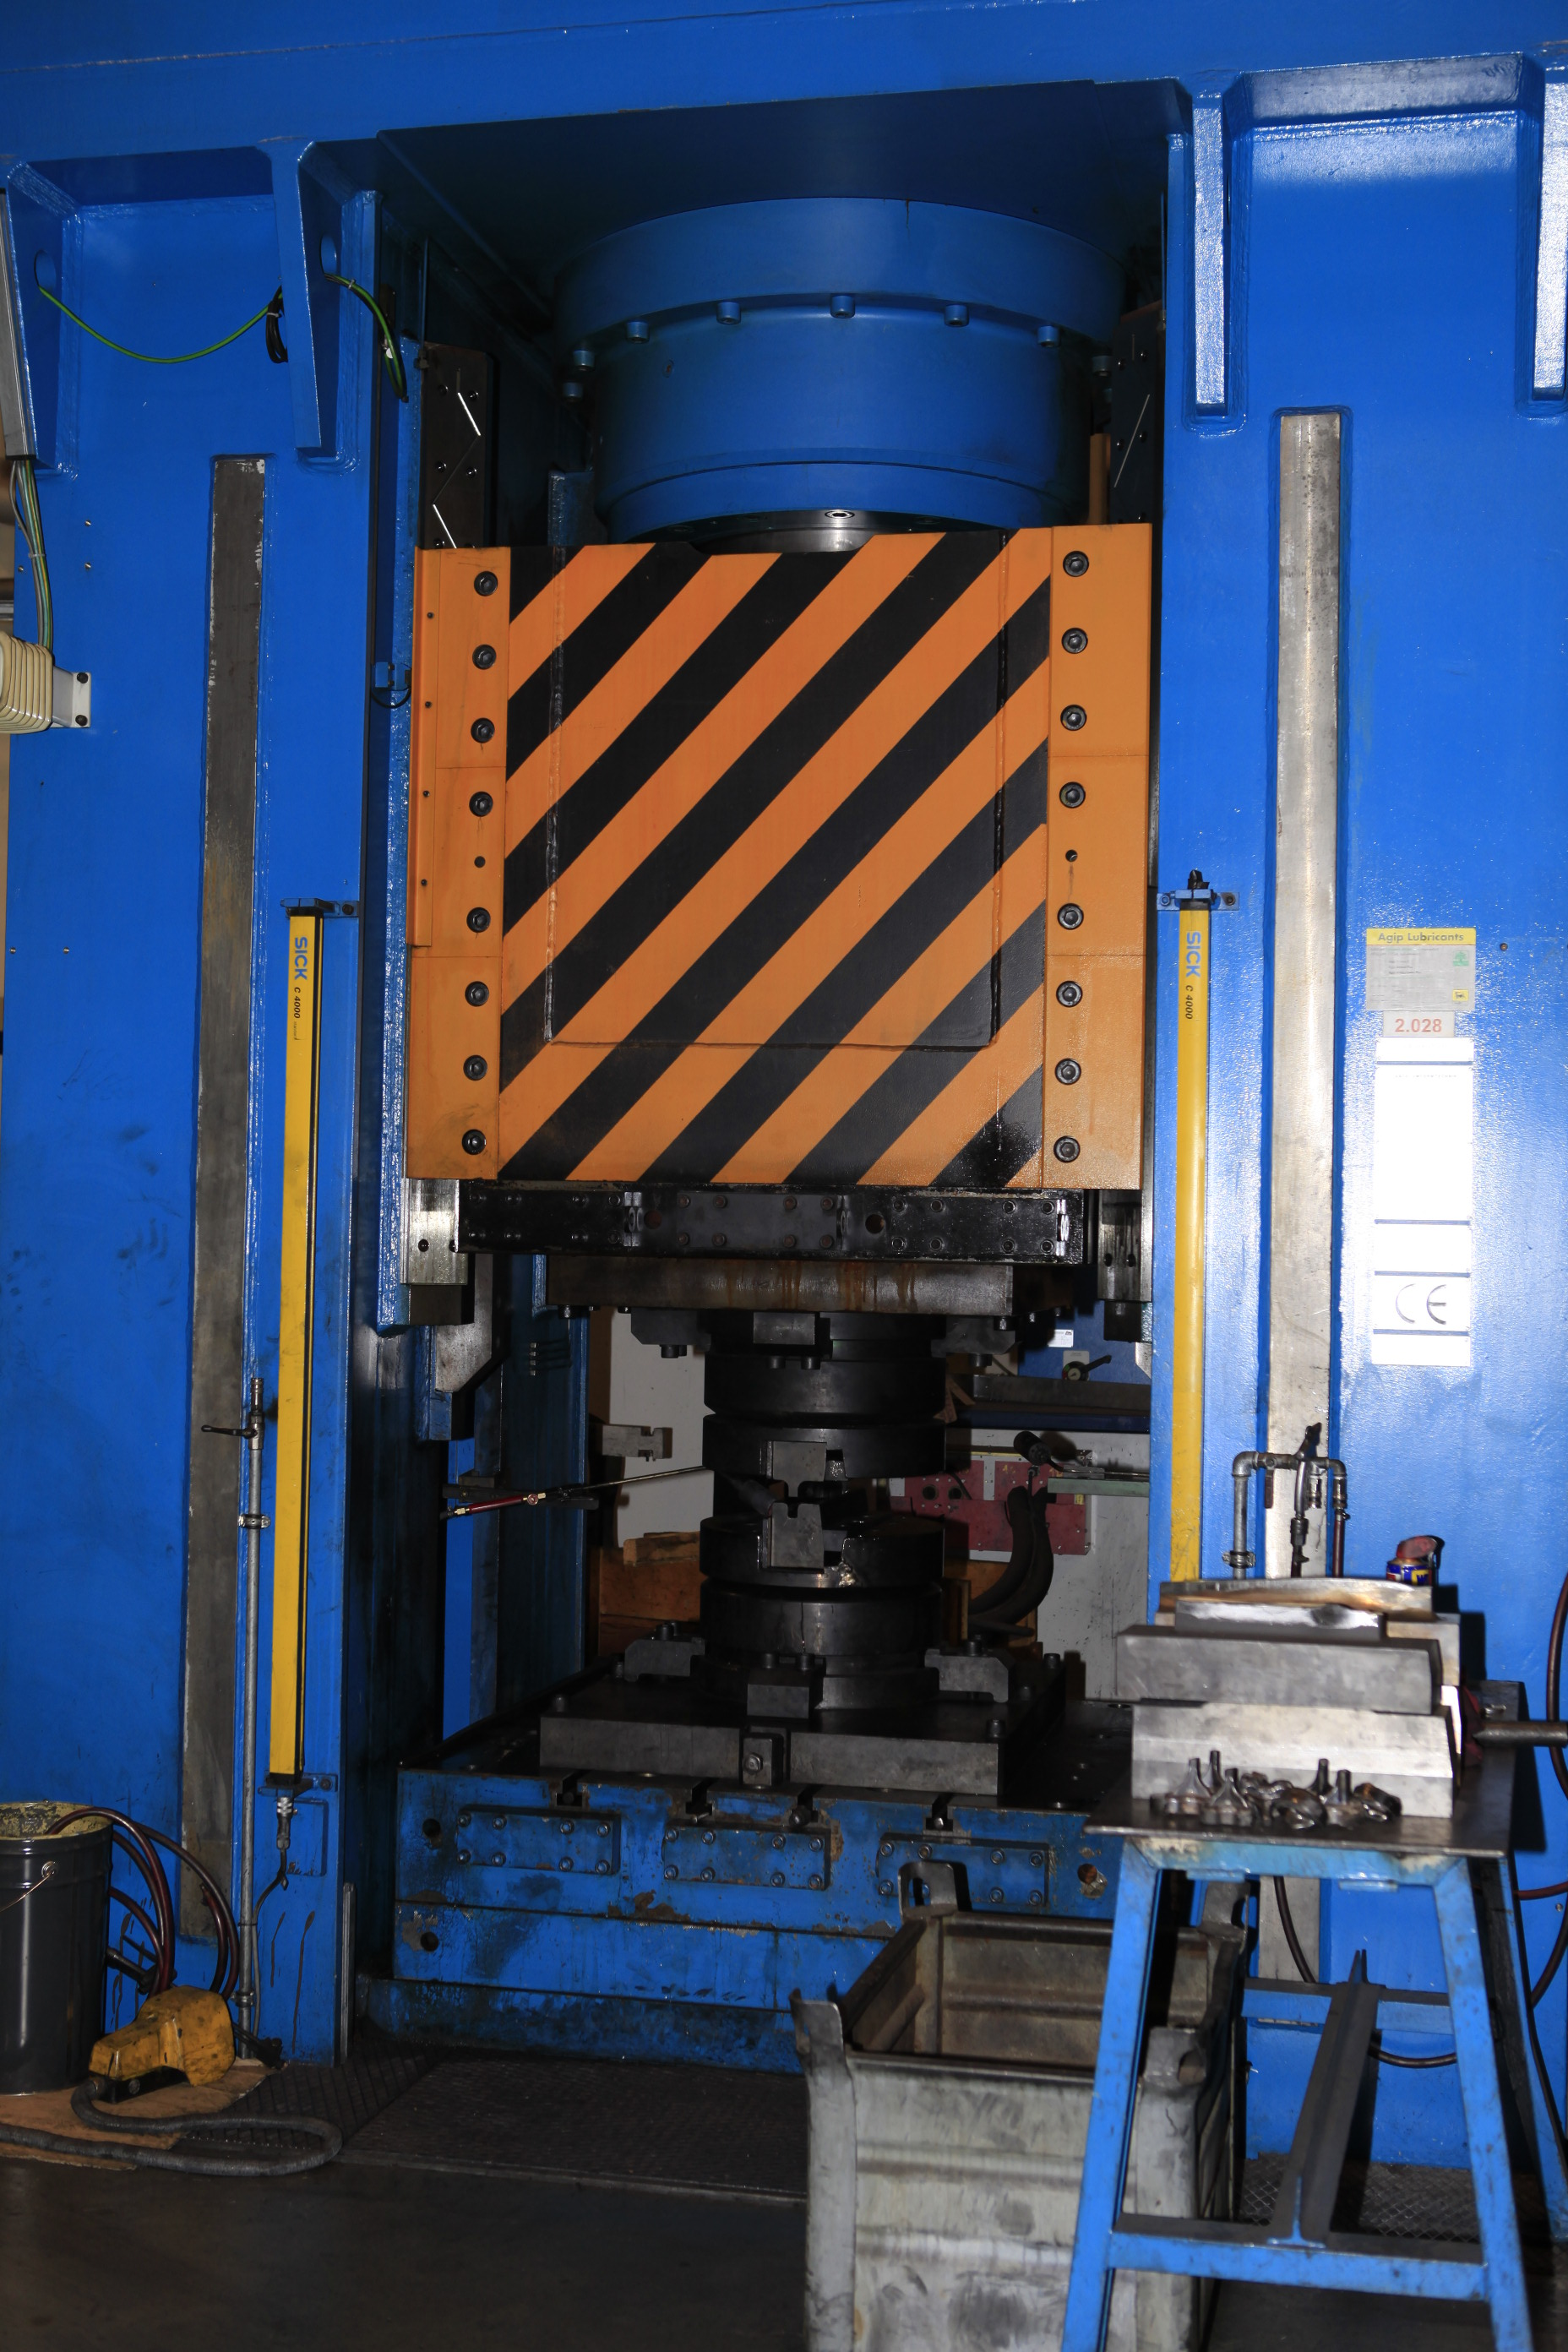
\includegraphics[width=\linewidth]{img/presse.jpg}
\caption{Presse de forgeage}
\label{fig:image3}
\end{center}
\end{minipage}
\end{figure}

Les liaisons entre coulisse 2 et coulisse 3 puis entre coulisseau et bâti sont des liaisons glissière.

\paragraph{Question 1:} Déterminer $\overrightarrow{V_{A \in 1/0}}$. En déduire $\overrightarrow{V_{A \in 2/0}}$.

\paragraph{Question 2:} Déterminer la direction de $\overrightarrow{V_{A \in 2/3}}$ et $\overrightarrow{V_{A \in 3/0}}$.

\paragraph{Question 3:} Déterminer la norme de $\overrightarrow{V_{A \in 3/0}}$.

\paragraph{Question 4:} Effectuer la même étude pour :
\begin{enumerate}
 \item $\theta_{10} = 0\textdegree$,
 \item $\theta_{10} = 45\textdegree$,
 \item $\theta_{10} = 90\textdegree$.
\end{enumerate}

\paragraph{Question 5:} Donner alors l'allure de la vitesse de 3 par rapport à 0 en fonction de $\theta_{10}$.

\newpage

\begin{figure}[!h]
\begin{center}
\vspace{5cm}
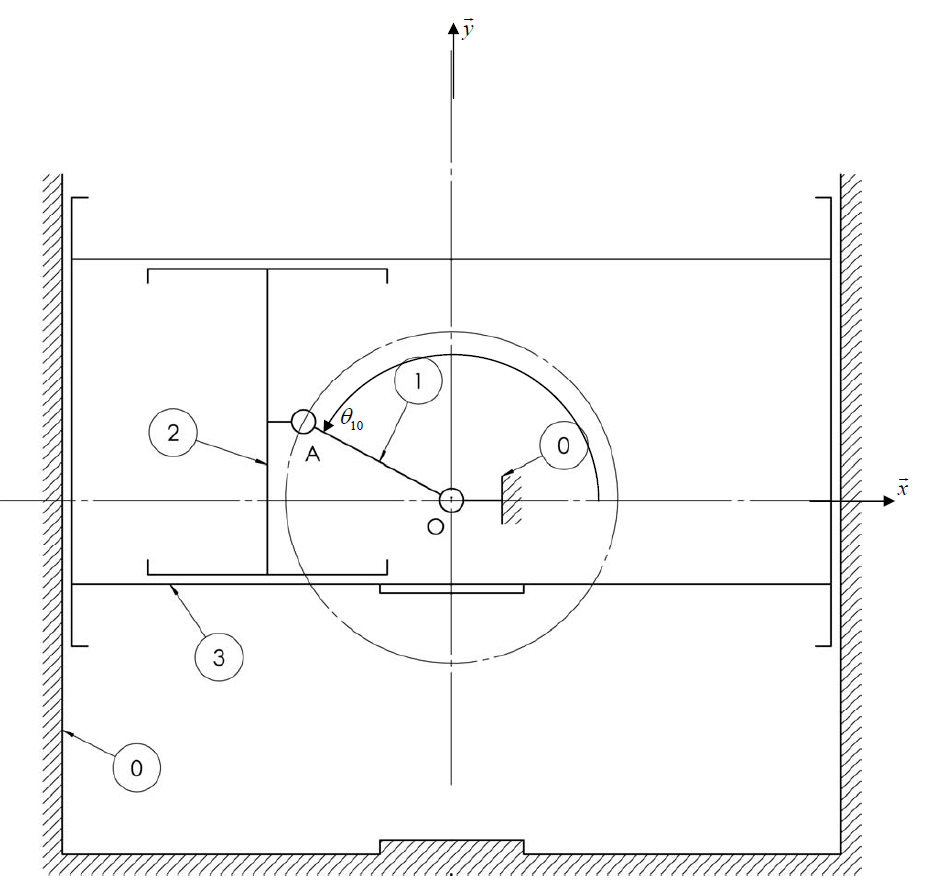
\includegraphics[width=0.7\linewidth]{img/presse_s.png}
\vspace{6cm}
\caption{Document réponse}
\label{fig:image4}
\end{center}
\end{figure}

\newpage

\section{Batteur de houle}

\begin{figure}[!h]
\begin{minipage}[c]{.6\linewidth}
Certains centres aquatiques ou laboratoires d'étude, figure \ref{fig:image5}, possèdent des piscines à vagues simulant les houles maritimes. Ces piscines comportent, sur un coté, un mécanisme appelé \og Batteur à houle \fg permettant de générer des vagues.

\centering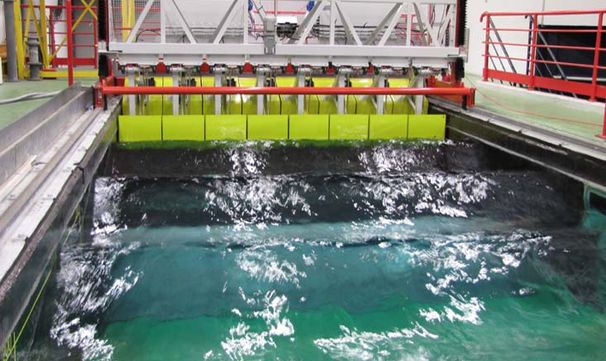
\includegraphics[width=0.8\linewidth]{img/batteur.jpg}
\caption{Bassin équipé}
\label{fig:image5}
\end{minipage}
\hfill
\begin{minipage}[c]{.35\linewidth}
\begin{center}
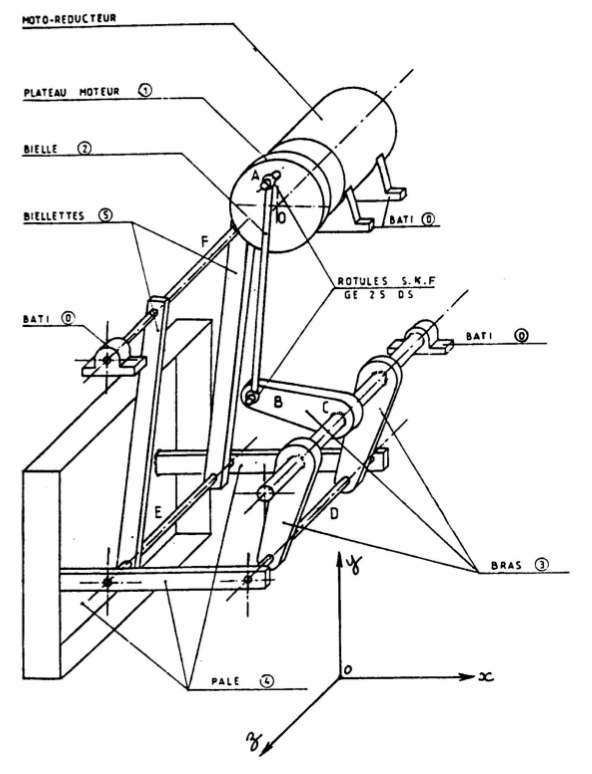
\includegraphics[width=0.9\linewidth]{img/Batteur1.png}
\caption{Bateur de houle}
\label{fig:image6}
\end{center}
\end{minipage}
\end{figure}

La vitesse d'entrée est la vitesse de rotation de la pièce 1 par rapport au bâti 0. 

Données:
\begin{itemize}
 \item $\|\overrightarrow{\Omega_{1/0}}\|=6 rad.s^{-1}$,
 \item $OA = 100mm$.
\end{itemize}

\paragraph{Question 1:} Déterminer $\overrightarrow{V_{A \in 1/0}}$. En déduire $\overrightarrow{V_{A \in 2/0}}$.

\paragraph{Question 2:} Déterminer la direction de $\overrightarrow{V_{B \in 3/0}}$. En déduire celle de $\overrightarrow{V_{B \in 2/0}}$.

\paragraph{Question 3:} Déterminer la norme de $\overrightarrow{V_{B \in 2/0}}$. En déduire celle de $\overrightarrow{V_{B \in 3/0}}$, puis celle de $\overrightarrow{V_{D \in 3/0}}$.

\paragraph{Question 4:} Déterminer la direction de $\overrightarrow{V_{E \in 5/0}}$. En déduire celle de $\overrightarrow{V_{E \in 4/0}}$.

\paragraph{Question 5:} Déterminer la norme de $\overrightarrow{V_{E \in 4/0}}$, puis celle de $\overrightarrow{V_{J \in 4/0}}$ et de $\overrightarrow{V_{K \in 4/0}}$.

\newpage

\begin{figure}[!h]
\begin{center}
\vspace{6cm}
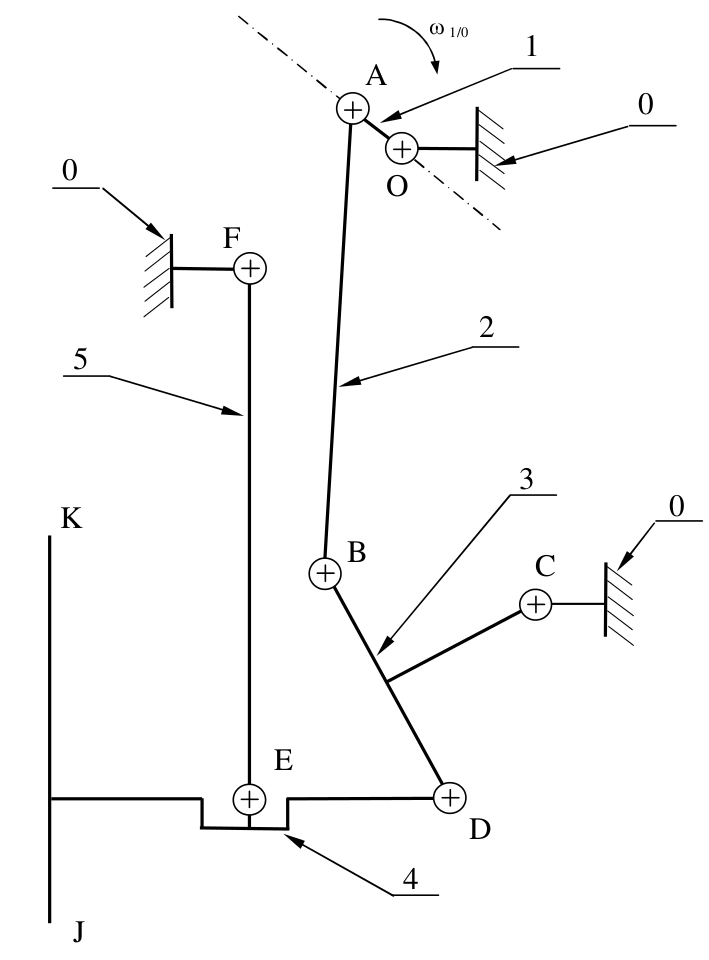
\includegraphics[width=0.6\linewidth]{img/Batteur_s.png}
\vspace{6cm}
\caption{Document réponse}
\label{fig:image7}
\end{center}
\end{figure}

\end{document}